% This must be in the first 5 lines to tell arXiv to use pdfLaTeX, which is strongly recommended.
\pdfoutput=1
% In particular, the hyperref package requires pdfLaTeX in order to break URLs across lines.

\documentclass[11pt]{article}

% Remove the "review" option to generate the final version.
% \usepackage[review]{emnlp2021}
\usepackage{emnlp2021}

% Standard package includes
\usepackage{times}
\usepackage{latexsym}

% For proper rendering and hyphenation of words containing Latin characters (including in bib files)
\usepackage[T1]{fontenc}

% This assumes your files are encoded as UTF8
\usepackage[utf8]{inputenc}
\usepackage{microtype}

% ======================================================================
% PEC For some reason the EMNLP templates put LH column line numbers on
% the right side. This switches them to the left side.
\usepackage[switch]{lineno} % default option is 'left
% ======================================================================

% PEC additions
\usepackage{graphicx}
\newcommand{\nk}[1]{\textcolor{green}{Nora: #1}}
\newcommand{\reworded}[1]{\textcolor{blue}{#1}}
\newcommand{\eat}[1]{}
\newcommand{\red}[1]{\textcolor{red}{#1}}
\newcommand{\blue}[1]{\textcolor{blue}{#1}}
\newcommand{\orange}[1]{\textcolor{orange}{#1}}
\newcommand{\green}[1]{\textcolor{ForestGreen}{#1}}
\newcommand{\teal}[1]{\textcolor{teal}{#1}}
\newcommand{\magenta}[1]{\textcolor{magenta}{#1}}
\usepackage{quoting}
\newenvironment{myquote}{                   % list without par spacings
  \parskip 0mm \begin{quoting}[vskip=0mm,leftmargin=2mm]}{
\end{quoting}}
\newenvironment{myquote2}{                   % list without par spacings
  \parskip 1mm \begin{quoting}[vskip=0mm,leftmargin=4mm]}{
\end{quoting}}
\newenvironment{ite}{                     % list without par spacings
     \parskip 0cm \begin{itemize} \parskip 0cm \parsep 0cm \itemsep 0cm \topsep 0cm}{
        \end{itemize}} %  \parskip 0cm}
\newenvironment{enu}{                   % list without par spacings
     \parskip 0cm \begin{list}{}{\parsep 0cm \itemsep 0cm \topsep 0cm}}{
       \end{list}} %  \parskip 0cm}
\newenvironment{des}{                 % list without par spacings
     \parskip 0cm \begin{list}{}{\parsep 0cm \itemsep 0cm \topsep 0cm}}{
       \end{list}} %  \parskip 0cm}
\newenvironment{myenumerate}{                   % list without par spacings
     \parskip 0cm \begin{enumerate}{\parsep 0cm \itemsep 0cm \topsep 0cm}}{
        \end{enumerate}} %  \parskip 0cm}
\newenvironment{myitemize}{                     % list without par spacings
     \parskip 0cm \begin{itemize}{\parsep 0cm \itemsep 0cm \topsep 0cm}}{
        \end{itemize}} %  \parskip 0cm}

% ======================================================================

% If the title and author information does not fit in the area allocated, uncomment the following
%
%\setlength\titlebox{<dim>}
%
% and set <dim> to something 5cm or larger.

\title{Enriching a Model's Notion of Belief using a Persistent Memory} 
% BeliefBanks: Adding Persistent Memory to Enrich a Model's Notion of Belief (?) \\
% What does My Model Believe? }

% Author information can be set in various styles:
% For several authors from the same institution:
% \author{Author 1 \and ... \and Author n \\
%         Address line \\ ... \\ Address line}
% if the names do not fit well on one line use
%         Author 1 \\ {\bf Author 2} \\ ... \\ {\bf Author n} \\
% For authors from different institutions:
% \author{Author 1 \\ Address line \\  ... \\ Address line
%         \And  ... \And
%         Author n \\ Address line \\ ... \\ Address line}
% To start a seperate ``row'' of authors use \AND, as in
% \author{Author 1 \\ Address line \\  ... \\ Address line
%         \AND
%         Author 2 \\ Address line \\ ... \\ Address line \And
%         Author 3 \\ Address line \\ ... \\ Address line}

\author{Nora Kassner, Hinrich Sch{\"u}tze \\
Center for Information and Language Processing \\
LMU Munich, Germany \\
\texttt{kassner@cis.lmu.de} \\ \And
Oyvind Tafjord, Peter Clark \\
Allen Institute for AI \\
Seattle, WA \\
\texttt{\{oyvindt,peterc\}@allenai.org} \\
}

\begin{document}
\maketitle
\begin{abstract}
% \nk{Regarding the title: I liked the Believe me...}
Although pretrained language models (PTLMs) have been shown to contain significant
amounts of world knowledge, they can still produce inconsistent answers to questions when probed,
even after using specialized training techniques to reduce inconsistency. As a result, it can be
hard to identify what the model actually
"believes" about the world. Our goal is to reduce this problem, so systems are 
more globally consistent and accurate in their answers. Our approach is to add a
memory component - a BeliefBank - that records a model's answers,
and two mechanisms that use it to improve consistency among beliefs. First, a reasoning
component - a weighted SAT solver - improves consistency by flipping
answers that significantly clash with others. Second, a feedback
component re-queries the model but using known beliefs as context.
We show that, in a controlled experimental setting, these two mechanisms
improve both accuracy and consistency. This is significant as it is a
first step towards endowing models with an evolving memory,
allowing them to construct a more coherent picture of the world.
\end{abstract}

\eat{
\red{Why experiments are slow:
\begin{itemize}
    \item calibration is a problem!!! When I extended the dataset the calibration seems to not work well. I changed it to a heuristic alternative which seems to work but that means I have to rerun all SAT solving experiments
    \item SAT solving takes per entity: 6 min
    \item each run of the full graph takes > 1h
    \item + 10 plants: 10 h
    \item + 20 incremental with random context: 20
    \item + 20 incremental with bm25 context: 20
    \item + 20 incremental with bm25 SAT solved context: 20
    \item + averaging over multiple splits maybe 5?: 20*4
\end{itemize}}

\red{What are the current issues:
\begin{itemize}
    \item If calibration is of F1 can still improve but it flips essential things from no-->yes and random things from yes-->no
    \item What kind of F1 should I report? Derivable facts (small test set but large improvements), gold facts (even smaller test set with good model performance and only small improvements, all IsA facts (might include a couple of wrong labels, large test set, only slight improvements as many nodes need more mutual exclusive connectivity)
    \item I have to filter plurals
    \item Do we expect the model to understand negation inside to context window?
\end{itemize}}
}

\section{Introduction}

% \vspace{-1mm}
\begin{figure}[t]
\centering
     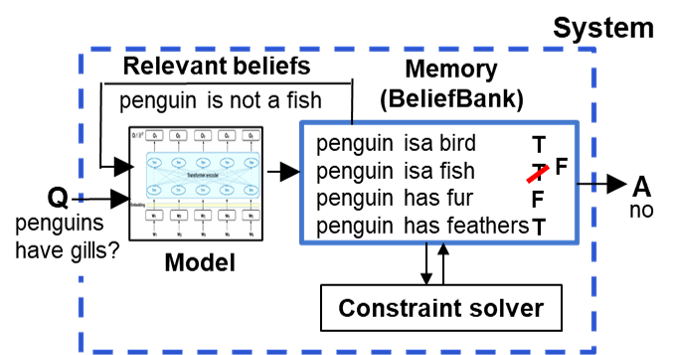
\includegraphics[width=1\columnwidth]{architecture2.png}	   % small figure
%      \vspace{-3mm}
\caption{The proposed architecture. The model's raw answers are stored in a
persistent memory (BeliefBank), and two mechanisms attempt to improve them:
(a) A {\bf constraint solver} flips beliefs that clash significantly with others
(b) A {\bf feedback} mechanism re-queries the model about those beliefs, but
uses relevant beliefs as the query context. We find both the consistency and accuracy
of the overall system improves. \label{architecture}}
% \caption{The proposed architecture. A memory layer (the BeliefBank)
% plus constraint solver improves the consistency of beliefs.
% Given a new question, relevant beliefs are recalled to help improve
% the model's answers, thus feeding more accurate results back into the BeliefBank.
% \label{arcuitecture}}
% \vspace{-3mm}
\end{figure}

How might we ascribe a notion of belief to a model? Prior work has shown that, while
pretrained language models (PTLMs) contain substantial world knowledge \cite{Petroni2019LanguageMA, roberts-etal-2020-much},
their answers to probing questions can be inconsistent \cite{Elazar2021MeasuringAI, ravichander-etal-2020-systematicity, Kassner2020NegatedAM},
% models have high question-answering (QA) accuracy \nk{should we specify that we are talking about “closed-book question answering” and refer to papers that show that PLMs are good at it? }, they can also be inconsistent in their answers, 
making it hard to pin down what a model actually ``believes'' about a proposition.
% How might we ascribe a notion of belief to a model? Prior work has shown that, while
% models have high question-answering (QA) accuracy \nk{should we specify that we are talking about “closed-book question answering” % and refer to papers that show that PLMs are good at it? }, they can also be inconsistent in their
% answers, making it hard to pin down what a model actually ``believes'' about a proposition.
Our goal is to reduce this problem by having systems provide more globally consistent
answers to questions.

Prior work on reducing inconsistency has focused on retraining the model itself to be
more consistent in its answers, e.g., \cite{Ribeiro2019AreRR,Li2019ALF}, but with imperfect results. We present an
alternative approach in which the model is unchanged, but an evolving, persistent memory
of beliefs - called the BeliefBank - is layered on top, and two mechanisms use it 
to improve consistency among beliefs. First a reasoning component - a weighted SAT solver -
flips beliefs that clash with others. Second, a feedback component re-queries the model
but using known beliefs as context, aiming for more accurate and consistent answers. 
Thus, the overall system attempts to build a more coherent representation of the
world from the model's raw answers, by ruminating on the answers seen so far.
This can also be viewed as assembling a simple ``mental model'' of the world \cite{JohnsonLaird1983MentalM} from
the noisy output of a raw PTLM.

\eat{
% I'm heartbroken to drop this paragraph!!!!! EMNLP perhaps?
In addition, 
just as the model helps populate the BeliefBank, we also show how beliefs in
the BeliefBank can improve the model's answers to future questions,
by using the most relevant beliefs as additional context for question-answering
(i.e., reminding the model of important facts pertinent to the new question).
These improved answers then feed into the growing BeliefBank, allowing the
overall system (model + BeliefBank) to continuously improve performance over
time, without retraining the model itself.
}

We explore this in a controlled experimental setting where 
both candidate facts and candidate constraints are provided. Candidate facts are simple
sentences that may be true or false, e.g., "An eagle is a bird" (T), ``An eagle is a mammal'' (F). Candidate constraints are between (variabilized) facts, e.g., ``?X is a bird $\rightarrow$ ?X can fly''. These allow us both to probe and measure improvement
in the system's consistency and accuracy, described shortly.

\eat{
\red{Delete/reword this paragraph} Our approach involves an interplay between a model's raw answers, and an
evolving memory - the BeliefBank - of beliefs based on the model's earlier answers
and a set of constraints that should hold. Model's answers contribute to the BeliefBank,
and the BeliefBank contribute new context to help with future question-answering by
the model. In between, a constraint system serves to identify and reduce inconsistency
among beliefs in the BeliefBank. Combined, this results in a system capable of
continuous improvement over time, opening new possibilities for dialog and
interactive teaching.
}

\red{List contributions}
We make the following contributions: i) We propose to augment a PTLM with a global memory - the BeliefBank to track a PTLM's "beliefs" ii) We compare two mechanisms of exploiting this BeliefBank - a reasoning and a feedback mechanism iii) We contribute a controlled dataset to measure a PTLM's consistency to given constraints. iv) We show that PLMs struggle with mutual exclusive constraints. v) Finally, we show that both mechanisms improve both overall accuracy and consistency on that dataset.

\section{Related work}

% \nk{Some more related work- perhaps fold into the below: \cite{Talmor2020TeachingPM}, knowledge in PLMS 
% \cite{Petroni2019LanguageMA,roberts-etal-2020-much} \cite{kassner-etal-2020-pretrained}}
% \red{Possibly cite \cite{Graves2016HybridCU} - the memory there is more like
% an opaque expansion of the original network. I'm inclined not to cite this though
% as it's old and not really relevant.}
\nk{some more related work to add:
\cite{Thorne2020NeuralD}
\cite{Camburu2020MakeUY}
% 2 more inconsistency papers: \citet{Camburu2020MakeUY}
% \citep{du2019consistent}
}


PTLMs are known to contain extensive world knowledge \cite{Petroni2019LanguageMA, roberts-etal-2020-much},
yet be inconsistent in their answers to probing questions \cite{ettinger-2020-bert, Kassner2020NegatedAM, ravichander-etal-2020-systematicity, Elazar2021MeasuringAI}.
While there has been some prior work on improving answer consistency, the primary approach
has been through modified model training. \citet{Ribeiro2019AreRR} improved consistency
by adding question paraphrases and question implications to the training data (data augmentation).
Others have trained models with (small) {\it sets} of examples with known constraints
between them, and included an additional loss term reflecting inconsistency among
set members during training \cite{Minervini2018AdversariallyRN,Li2019ALF,Asai2020LogicGuidedDA}.
However, the constraints are unused at test time (beyond what the model may have
internalized), and inconsistent answers are still produced.

For problems requiring a structured answer, e.g., predicting a sequence of
state changes, domain-specific constraints have been used to downgrade/block
answers that violate them \cite{Tandon2018ReasoningAA,Du2019BeCI}. This
encourages consistency within a single answer structure, but not among
different answers, our goal here.

% Concerning improving global consistency using constraints,
In the area of knowledge graph construction,
% , where individual extractions may be noisy, 
\citet{Pujara2013KnowledgeGI} define ``knowledge graph identification''
as the task of building a maximally consistent knowledge graph given noisy facts
and their extraction confidences, and ontological constraints between them.
They develop a solution use probabilistic soft logic (PSL) \cite{Broecheler2010ProbabilisticSL}
as their constraint reasoner. 
Similarly \citet{berant2010global} learn the globally
optimal set of entailments between a large database of candidate
entailment pairs (with associated confidences), by applying
a global transitivity constraint (X$\vdash$Y \& Y$\vdash$Z $\rightarrow$ X$\vdash$Z)
using Integer Logic Programming. 
Our constraint solver performs an analogous
function in our architecture, using the Z3 SAT solver (Section~\ref{??}).
\red{Say how we are different/go beyond.}

In the area of formal knowledge-bases (KBs), efficient algorithms
have been developed for detecting, measuring, and resolving inconsistency
\cite{hansen2000probabilistic,andersen2001easy,Thimm:2009d,muino2011measuring,Thimm:2013}.
Our contribution is to leverage some of these methods for PTLMs,
adding a reasoning capability that the PTLMs alone lack.

An important part of our contribution is the use of a dynamic, persistent memory.
While there are neural architectures that include an associated memory,
e.g., \cite{Henaff2017TrackingTW,Sukhbaatar2015EndToEndMN}, these components
typically play the role of a short-term working memory to help computation.
In contrast, our BeliefBank memory layer is a persistent, long-term memory of
explicit beliefs.

\eat{
% \subsection{PLMs and knowledge}
\subsection{Faithfulness}
\citet{subramanian-etal-2020-obtaining}
introduce the concept of module-wise faithfulness, a systematic evaluation of faithfulness in neural module networks for reasoning. We show that naive training does not produce faithful modules and propose several techniques to improve module-wise faithfulness. 
}
\eat{
\subsection{Inconsistencies in KGs}
(copied from old paper, need rewrite)
Consistency in KBs has been
studied in theoretical frameworks in the context of the
satisfiability problem and KB construction, and efficient
algorithms for detecting inconsistencies in KBs have been
proposed \cite{hansen2000probabilistic,andersen2001easy}.
Other work aims to quantify the degree to which KBs are
inconsistent and detects inconsistent statements
\cite{Thimm:2009d,muino2011measuring,Thimm:2013}.
% \cite{zhang2020need} showed that capturing factual knowledge inside PLMs is a specially resource hungry task.
}

\section{Task}

\subsection{Beliefs}

What does it mean to believe a proposition, say p = eagles are birds? In general, a system can
be said to (appear to) believe something if it acts as if it were true. In the specific
context of a QA system, we would expect it to produce answers consistent with p (and
its other beliefs). Pragmatically, we expect the system to (a) give a consistent answer to
different paraphrases of the question "p?" ("Are eagles birds?", "Is an eagle a type of bird?", ...),
and (b) give correct answers about implications of p ("Eagles lay eggs", "Eagles have feathers", ...),
conditional on the system knowing such implications and how to apply them.
% For example,
% if a system believes eagles are birds, and knows birds lay eggs (plus the rule of inheritance),
% we would expect it to answer "yes" to a question about whether eagles lay eggs.
Of course, a system may not perfectly answer such implications as the implications
may have exceptions, or the system may not be a perfect reasoner.\footnote{Similarly,
people do not always behave fully consistently with their professed beliefs.}.
Thus, to the external observer, there are {\it degrees} to which a system acts as if it
believes something.
% (Note this is distinct from a system's internal confidence in a belief).

\eat{
\red{Possibly delete this paragraph if too repetitive.} 
As has been shown elsewhere, language models (LM) can be inconsistent in their answers,
suggesting they have a rather weak notion of belief, in the sense described above.
To strengthen this, we add a dynamic memory component - the BeliefBank - on top of
the model to track and modify beliefs. We use the phrase ``the {\bf system}'' to refer
to the combined model plus belief bank. Our goal is to create a system with
a stronger notion of belief (i.e., more consistent and accurate) than the underlying LM inside it.
}

\subsection{Task Definition}

Our goal is to ascribe a stronger notion of ``belief'' to a system that includes a model $M$,
by improving the consistency and accuracy of its answers (compared with $M$). To measure
this we consider a true/false probing task, where we are also given a set of
constraints between answers:
\begin{myquote}
{\bf Given:}
\begin{ite}
\item a set of {\bf sentences} $S$ 
\item a set of {\bf constraints} $C(S)$ between (the truth values of) sentences in $S$, each annotated with a weight $w_i$ (A penalty $w_i$ is applied if $c_i$ is violated)
\item a {\bf model} $M$ that takes as input a True/False (NL) question $Q$ and optionally an (NL) context $X$, and predicts a True/False answer $A$ with confidence score $F$
\end{ite}
{\bf Predict:}
\begin{ite}
\item the True/False labels for $S$, so as to maximally improve accuracy (with respect to gold labels) and
   consistency (minimize total penalties of constraint violations) compared with model $M$'s raw answers
\end{ite}
\end{myquote}
% As a toy example from Figure~\ref{example}, $S$ = \{penguin is a bird, penguin is a fish, penguin has fur, penguin has feathers, penguin has gills}, $C(S)$ = \{?X isa bird $\rightarrow$ NOT ?x isa fish, ?X isa fish $\rightarrow$ NOT ?x isa bird\},
% and the raw model $M$'s answers are \{T,T(wrong),F,T,T(wrong)\}. 
\red{Move later} As our dataset class distribution (described shortly) is unbalanced, with significantly fewer True than False
answers, we measure accuracy using F1 (over True questions) to avoid scores being dominated by negative
answers.



\section{Approach}

% Our goal is to ascribe a stronger notion of ``belief'' to a model,
% by improving the consistency and accuracy of its answers. 
Our approach is to add a
memory layer, called the {\bf BeliefBank}, on top of the model to globally 
track beliefs. Two mechanisms are then used to modify BeliefBank beliefs, namely
(a) {\bf constraint reasoning} and (b) re-asking queries augmented with {\bf feedback} from the BeliefBank.

\subsection{Definitions \label{definitions}}

\eat{
\nk{Some comments on these definitions below: Can we find an alternative to $\textrm{tf}_i$? In our case the constraint is if X is True then Y is True/False. In general this could be also If X is False then Y is True/False. We could denote the belief as $\neg$ $s_i$/$s_i$ with an associated $w_i$ strength}

\red{Pete: I'm not quite comfortable with describing $s_i$ as an ``assertion''. An assertion is a statement
of fact or belief, but the $s_i$ themselves are just neutral sentences with no associated claims of truth or falsehood.
We could use the word ``statement'', if ``sentence'' sounds too syntactic (though as we've discussed,
the precise wording {\it is} important). Or perhaps each $s_i$ is (a sentence expressing) a statement about the world.?
Or each $s_i$ is (a sentence expressing) a possible assertion about the world?}

\red{Pete: Also, we do in fact reason with the truth values T/F of propositions, as illustrated in
Figures~\ref{architecture} and ~\ref{progression}, and in the SAT solver, so I wonder if we should call out the truth value as a 
separate entity. It seems a little strange to define $s_i \in S$ as a possible assertion, but then also say
$s_i$ is a belief. It shouldn't be both! I suppose we could say a belief is a (possibly negated) $s_i$ in the BeliefBank....}
}

\noindent Let
\vspace{-2mm}
\begin{ite}
  \item a {\bf belief} $b_i$ be a triple ($s_i$,$l_i$,$w_i$), where 
     \begin{ite}
     \item $s_i$ is a sentence $\in S$ % expressing a proposition about the world
      \item label $l_i \in$ \{T,F\} denotes the system's True/False belief about the truth of $s_i$
     \item weight $w_i$ is a number $\in [0,1]$ representing the system's strength of that belief
    \end{ite}
 For example:
 \begin{quote}
{\it      ("a poodle is a dog", T, 0.9) }
 \end{quote} 
 denotes the belief (strength 0.9) that "a poodle is a dog" is a true statement (T).
  \item a {\bf BeliefBank} $B(S)$ = a set of beliefs over assertions $S$ = $s_1,...,s_n$
 \item For notational convenience, we denote the believed truth $l_i$ of $s_i$ according to $B(S)$ as $bel(s_i,B(S))$
 \item a {\bf constraint} $c_i$ = a 4-tuple of the form 
($s_i \rightarrow s_j, l_j, w_i$)
where 
\begin{ite}
\item $s_i,s_j$ are sentences $\in S$, 
\item $l_j \in$ \{T,F\} denotes the expected truth of $s_j$ if $s_i$ is true,
\item $w_i$ denotes the strength of that expectation (a penalty $w_i$ is applied if it is violated). 
\end{ite}
For convenience, we allow a shared variable X to be used in $s_i,s_j$, allowing a set of grounded
constraints to be expressed in a single statement, e.g.
\begin{myquote}
{\it (``X is a dog'' $\rightarrow$ ``X has a tail'', T, 0.8) }
\end{myquote}
expresses that if something is a dog, then it should (T) have a tail, with a penalty of 0.8 applied if
it does not.
\item A {\bf constraint graph} $C(S)$ = a set of constraints $c_i$ over assertions $S$ 
% \red{This is problematic
% as $S$ in constraints (now) contain a variable ?X. So is $S$ sentences with or without variables?}
\end{ite}
Given a set of beliefs $B(S)$ about $S$ and a set of constraints $C(S)$, we measure the {\it consistency}
of those beliefs using the weighted sum of all violated constraints. Dropping the $S$ parameter for convenience:
 \begin{myquote}
  consistency(B,C) = \\
\hspace*{2mm}  $- \sum_{c_i \in C} \{~ w_i ~ | ~ c_i = (s_i \rightarrow s_j, l_j, w_i )       ~\& \\
\hspace*{18mm}  bel(s_i,B) ~ \& ~ bel(s_j,B) \neq l_j ~ \}$
\end{myquote}
i.e., for each constraint $c_i$, if the system believes the constraint's condition ($bel(s_i,B)$), but does not
believe the expected truth of the conclusion ($bel(s_j,B) \neq l_j$), then the system is penalized by the (negative of)
the constraint's weight $w_i$. Although this measure is dependent on the constraints and penalties used,
it allows us to perform {\it comparative} experiments with different systems.


\begin{figure}[t]
\centering
     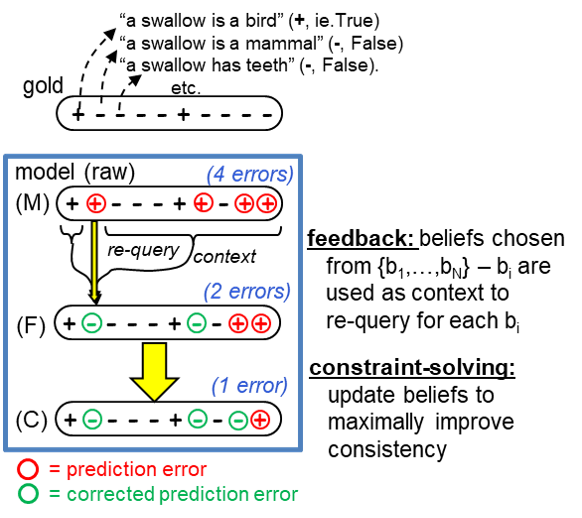
\includegraphics[width=1\columnwidth]{progression.png}	   % small figure
%      \vspace{-3mm}
\caption{Simplified illustration of iteratively improving the BeliefBank (oval). +/- denote true/false predictions for 10 facts about swallows. The model alone makes 4 prediction errors (M). Re-querying for those beliefs using other selected beliefs as context ({\bf feedback}) fixes 2 of those errors (F). Running {\bf constraint solving} on the updated BeliefBank fixes another error (C), resulting in just 1 error in the final BeliefBank. Here, the sequence is Model $\rightarrow$ Feedback $\rightarrow$ Constraints. We also evaluate other sequences (Table~\ref{results}).
\label{progression}}
% \caption{Simplified illustration of how the BeliefBank (oval) improves with time. +/- denote true/false predictions for 10 facts about swallows. The model alone makes 3 prediction errors (M). Alternatively, the model predicts batch1, making 1 error (A); using batch1 as context for batch2 results in only 1 new error (B); constraint solving fixes another error (C), resulting in just 1 error in the final BeliefBank (C).
% \label{progression}}
% \caption{Simplified illustration of how the BeliefBank (oval) improves with time. +/- denote true/false predictions for 10 facts about poodles. \nk{This example is a bit misleading. The raw answers are usually good with correct positive. A better example would be: a boa is a snake, a snake is a squamate, squamate is not a mammal, a boa is a mammal} The model alone makes 4 prediction errors (M). Alternatively, the model predicts batch1, making 2 errors (A); constraint solving fixes one (B); using batch1 as context for batch2 results in only 1 new error (C); constraint solving again fixes another error (D), resulting in just 1 error and greater consistency in the final BeliefBank (D). \label{progression}}
\end{figure}

\subsection{Methods}

We evaluate two methods for improving the BeliefBank's accuracy and consistency:
% using the constraints:
\begin{des}
\item[{\bf Constraint solving:}] Given a model $M$'s answers (with confidences) in the BeliefBank, a constraint
solver seeks to reduce constraint violations by potentially flipping answers that maximally clash
with other answers. 
% The answers in the revised BeliefBank are taken as the system's {\it overall} answers to questions.
\item[{\bf Feedback:}] Beliefs are checked by re-querying the model, but additionally
using relevant other beliefs as context for those (re-)queries. 
% Given a new question $q_{n}$, relevant beliefs in the BeliefBank are
% provided as additional input (namely as context) to help it answer $q_{n}$,
% to see if this improves the model's answer.
\end{des}
\vspace{1mm}
Figure~\ref{architecture} shows these components, and 
Figure~\ref{progression} illustrates how they can iteratively improve the BeliefBank.
In Figure~\ref{progression}, there there are 10 beliefs of interest about swallows. When probed about these, the raw model 
gets 4 of these wrong, including inconsistently believing that a swallow is both a bird and a mammal
(see (M) in Figure~\ref{progression}). Applying feedback, we re-ask the model the 10 questions but adding 
in the most relevant known beliefs as context for those (re-)queries. The BeliefBank is updated with
these new answers, fixing 2 of the errors (F). We then run the constraint solver over the BeliefBank,
resulting in one answer being flipped (question 9, from T to F), thus fixing another error (see (C)). 
The final BeliefBank has just 1 error and greater consistency.  As we describe later, we also
evaluate other orders of update (e.g., first constraint-solving then feedback) to identify which
is most effective. Note that updates can also 
introduce new errors (not shown in Figure~\ref{progression}), so improvement is not guaranteed. 

\subsubsection{Constraint Solving}

Given a set of beliefs and constraints, the constraint solver has two competing objectives: (a) flip 
beliefs so as to minimize constraint violations (b) don't flip beliefs, so as to preserve
the model's raw beliefs, i.e., minimize conflict between the model and BeliefBank. 
To implement this tradeoff, the model's beliefs are themselves treated as just
another constraint, e.g., the belief "a poodle is a dog" (weight 0.9) is treated as a constraint
"a poodle is a dog", with penalty 0.9 if it is violated (i.e., labeled as false by the constraint solver).
To balance the two objectives (a) and (b), the belief weights are scaled by a learned hyper-parameter $\lambda$,
trained on the training part of our dataset (Section~\ref{dataset}).

To implement constraint solving, we translate the task into a {\it weighted SAT} (satisfiability) problem $P$,
for which efficient algorithms with guarantees exist. Each belief becomes a weighted assertion in $P$, e.g.,
the belief ("a poodle is a dog", T, 0.9) is expressed in SAT syntax:
\begin{myquote2}
{\it 0.9 "a poodle is a dog"}\footnote{In practice, strings are replaced with numeric identifiers in SAT syntax, but for clarity we leave them as strings here.}
\end{myquote2}
while the constraint ("a poodle is a dog" $\rightarrow$ "a poodle has a tail", T, 0.8) is expressed:
\begin{myquote2}
{\it 0.8 "a poodle has a tail"  {\bf -}"a poodle is a dog"}
\end{myquote2}
(literally: a poodle has a tail OR NOT ("{\bf -}") a poodle is a dog). 
We then apply the solver Z3 \cite{??} to $P$, which outputs a set of truth assignments for all individual 
sentences in $P$ so as to minimize the weighted sum of violations. If the truth assignment of any sentence
has changed, the BeliefBank is correspondingly updated. \red{How do we update the weights?}.

% To find the optimal solution to the constraint equations, we convert the problem into a weighted SAT problem,
% and then use the Z3 SAT solver to find the optimal truth assignments to the beliefs. \red{Details are in
% Appendix~\ref{??}}.

\subsubsection{Feedback}

Feedback involves re-asking the model a question, but with the benefit
of knowing answers to related questions. To use these answers in the re-query,
selected beliefs are added to the query context before re-asking the model.
(Note that the selected beliefs are not guaranteed to be correct, of course).
Our conjecture is that if the model is explicitly reminded of relevant beliefs when answering a new question,
it will answer the question more accurately and consistently.
For example, in Figure~\ref{example}, when asked "Do penguins have gills?", our model $M$ incorrectly answers "yes".
But if reminded that penguins are not fish, by asking: "Penguins are not fish. Do penguins have gills?" 
the model now correctly answers "no". 

We evaluate three policies for choosing which beliefs to feed back to $M$ when re-asking question $Q$:
\begin{enu}
\item[1.] randomly selected from the BeliefBank
\item[2.] most similar, using the BM25 information retrieval ranking function \cite{bm25}
\item[3.] most confident (``core'') beliefs about the queried entity $e$, ... \red{explain}
\end{enu}
In all cases, three beliefs are selected (empirically found to be most effective).

\section{Dataset \label{dataset}}

\red{Still to do a pass over}

We create a dataset to test our approach in a controlled way, allowing us to perform systematic experiments to evaluate behavior.
The dataset is a collection of constraints derived from ConceptNet. In order to query whether the model is consistent and accurate, we use manually defined templates to query each sentence. We then evaluate the model's predictions on a test set of grounded facts.

\subsection{Constraints}
A {\bf constraint template} $t_i$ is a generalized constraint, namely a 4-tuple of the form
\begin{myquote} \centering
($\textrm{if}_i \rightarrow \textrm{then}_i, \textrm{tf}_i, p_i$)
\end{myquote} 
where $\textrm{if}_i, \textrm{then}_i$ are sentences containing a single, shared variable X, e.g.,
\begin{myquote} \centering

``X is a dog $\rightarrow$ X has a tail.''
\end{myquote}
If $\textrm{if}_i$ is true, \textrm{then} $\textrm{tf}_i \in$ \{True,False\} denotes the expected truth of $\textrm{then}_i$, 
with penalty $p_i$ if it is not.

\noindent
The dataset contains two kinds of constraints:
\begin{des}
\item[{\bf positive implications:}] ($\textrm{tf}_i$ = True), e.g.,``X is a dog $\rightarrow$ ?X has a tail.''
\item[{\bf mutual exclusivity:}] ($\textrm{tf}_i$ = False), e.g.,
``X is a dog $\rightarrow$ [$\textrm{tf}$=FALSE] X is a bird.'',
and ``X is a bird $\rightarrow$ [$\textrm{tf}$=FALSE] X is a dog.'', to
express that an entity cannot be both a dog and a bird at the same time.
% These are expressed as a pair of constraint templates each with $\textrm{tf}_i$ = False:

\end{des}
Positive implications were gathered from a filtered subset of ConceptNet triples.  We only consider English triplets with weights larger than 1.0. To gather these triplets we define a relevant entity set of entities with at least X number of occurrences. For these entities we collect all facts involving the 6 relations: IsA, HasA, MadeOf, PartOf, HasProperty, CapableOf and generate all possible transitive implications. For example, the ConceptNet triple (dog, HasA, tail) gives rise to the constraint (X, IsA, dog)$\rightarrow$ (X, HasA, tail).
We then manually filter theses constraints for factual correctness to exclude wrong implications like \red{XXX}. Finally, we use crowdsourceing to validate these constraints, see \ref{section:penalties}.

\eat{Mutual exclusivities were gathered from a filtered subset of the WordNet taxonomy,
based on the approximation that (generally) siblings in the WordNet noun hierarchy
are mutually exclusive \red{elaborate}.
}

Mutual exclusivities are gathered by deriving IsA-based hierarchy from the ConceptNet data based on the approximation that (generally) siblings in the noun hierarchy
are mutually exclusive. We enhance these exclusivities by WordNet hierarchy.


We collected 13,000 constraint templates in this fashion (1760 implications, \red{X} mutual
exclusivities).

\subsection{Constraint Strength}
\label{section:penalties}
We used a combination of crowdsourcing and calibration to assign a reasonable
constraint weight $w_i$ to each constraint. Workers were shown each
template and asked to judge if the implication held always/usually/sometimes/rarely/never with raw scores 4/3/2/1/0. This scoring procedure is used for forward implications as well as in the backwards direction. Backwards evidence is needed to prevent the SAT solver from flipping all answers to "no" which would result in perfect consistency but low accuracy. Rather than an actual implication, the backwards direction is evidence for a sentence to be true, e.g., "X has feathers.", "X has wings." and "X has two legs." accumulates to strong evidence for "X is bird." Three workers independently scored each template and the scores averaged.

\nk{Just a note for a modification for the next iteration of this: The backwardsscore is very ugly and I would like to get rid of it. I wonder if it is possible to do the calibration in a way that flipping "yes" to "no" needs very strong evidence.}


\subsection{Test set}
Given the constraint set, we can create a {\bf grounded} test set. \eat{by instantiating X with a particular entity, e.g., ``poodle'' (resulting in 200 
sentences and 13000 constraints about poodle).} 
To assign True/False labels to the
sentences, we identify and manually annotate the leaf sentences in the constraint DAG,
and then use the constraint rules to infer True/False labels for other sentences.
This provides ``silver'' labels for all the sentences, silver because constraint
rules may have exceptions in the real world for particular individuals (e.g.,
penguins don't fly). \nk{I would cut the example with the penguin and rather say somewhere else that we do not consider exceptions} For a given slice, we denote the sentences as $S$ and
the constraints about them as $C(S)$.

We repeat this for 20 \red{??} entities (10 animals, 10 plants), resulting
a final test set containing {\bf ?? silver facts} (sentences + True/False labels).
\eat{Note that each slice is independent and can be processed separately.
As described shortly, we perform our experiments with each slice in turn
and average results.}

\subsection{Calibration}
The raw scores were then calibrated by sigmoid-scaling, using a
grid search over slope and shift to identify the scaling hyper-parameters. We use a small set of seven entities and their grounded test set for calibration and maximize F1.   We also calibrate the relative weight of the model's beliefs and the constraints, and the relative weight of the forward, backwards and mututal exclusivities. \nk{Should I put more details in the Appendix?}

\subsection{Query and sentence templates}

In order to query the model for its belief we manually define template queries for each relation, e.g., for the IsA relation the template query "Is X a Y?" is used.
These template queries are then instantiated for each sentence of the constraint set by filling in the relevant objects Y, e.g., "Is X a dog?".

We then query the model's beliefs involving an entities of the test set by filling in the subject slot X, e.g., "Is a poodle a dog?".

We also define an additional set of sentence template, e.g., "X is Y." which is used to feed back beliefs into the context window of the model.



\eat{\subsection{Templates}

We collect all the unique variabilized sentences in the constraints together,
resulting in 200 \red{??} sentence templates, e.g., ``?X is a dog.''.
}


\section{Model}

The fixd model $M$ that we use for our experiments is the multi-angle QA system MAQAw \cite{arc-da}.
MAQAw is a derivative of UnifiedQA, a state-of-the-art T5 model fine-tuned on $\approx$400k question-answer pairs.
MAQAw was then 
further fine-tuned on several thousand science questions and trained on different permutations of inputs and outputs
(e.g., query Q + context C $\rightarrow$ answer A; CA $\rightarrow$ Q; etc.). 
To query the model's beliefs we pose the query and let the model chose between the two answer options "yes" and "no".
MAQAw outputs an answer probability...
NOTE this model is fixed for our experiments here.


\begin{table*}
\centering
{\small
\begin{tabular}{|l|ll|ll|ll|} \hline
Results after seeing \% of data $\rightarrow$ & \multicolumn{2}{|c|}{\bf 10\%} &
\multicolumn{2}{|c|}{\bf 50\%} &
\multicolumn{2}{|c|}{\bf 100\%} \\
Accuracy (F1), Consistency $\rightarrow$ & F1 & Con & F1 & Con & F1 & Con\\ \hline           
model (raw) & & & 74 & 77 & 74 & 76 \\
model + constraints & & & & & 88.5 & 100 \\
model + feedback (random)&  & & $\approx$85  & $\approx$89  &  &  \\
model + feedback (relevant for query constraints) & & & $\approx$88 & $\approx$91 & & \\\hline
%model + constraints + feedback (relevant for query + flipped)&&&87&90 & & \\\hline
% model + feedback (random positive) &&&&\\
% model + feedback (most confident) + constraints &&&& \\\hline
\end{tabular}
}
\caption{Results after seeing different proportions of data.
{\bf model (raw)} are scores for the model stand-alone.
In {\bf model + constraints}, the constraint solver is run over all
the raw answers so far. In {\bf model + feedback}, questions are re-asked
using context selected from the other raw answers so far. In {\bf model + feedback + constraints},
the constraint solver is additionally run on the answers with feedback. 
\label{results}}
\end{table*}

\begin{table*}
\centering
{\small
\begin{tabular}{|l|ll|ll|} \hline
Results after seeing $\rightarrow$ & \multicolumn{2}{|c|}{\bf batch1} &
\multicolumn{2}{|c|}{{\bf batch2}} \\
Accuracy (F1), Consistency $\rightarrow$ & F1 & Con & F1 & Con\\ \hline           
model (raw) & 74 & 77 &74 & 75 \\
model + constraints & 89&100& 88&100\\
model + feedback (random)& - & - & 85 & 89\\

model + feedback (relevant for query constraints)&-&-&88&91\\\hline
%model + constraints + feedback (relevant for query + flipped)&&&87&90\\\hline
model + feedback (random positive) &&\\
model + constraints + feedback (most confident) &&\\\hline
\end{tabular}
}
\caption{(old table)}
\end{table*}

\eat{\begin{table*}
\centering
{\small
\begin{tabular}{|l|ll|ll|ll|ll|} \hline
Results after seeing $\rightarrow$ & \multicolumn{2}{|c|}{\bf batch1} &
\multicolumn{2}{|c|}{+ {\bf batch2}} &
\multicolumn{2}{|c|}{+ {\bf batch3}} &
\multicolumn{2}{|c|}{+ {\bf batch4} (all)} \\
Accuracy (F1), Consistency $\rightarrow$ & F1 & Con & F1 & Con & F1 & Con & F1 & Con \\ \hline           
model (raw) & 48 & 76 & 28 & 79 & 42 & 75 & 44 & 72\\
model + constraints & & & & & & & & \\
model + feedback (bm25) & 48 & 76 & 39 & 92 & 48 & 78 & 58 & 86\\
model + feedback (random) & 48 & 76 & 42 & 94 & 56 & 86 & 56 & 81\\
model + constraints + feedback (most confident) & & & & & & & & \\
model + constraints + feedback (relevant for query) & & & & & & & & \\
model + constraints + feedback (relevant for query + flipped) & & & & & & & & \\\hline
\end{tabular}
}
\caption{{\bf model (raw)} shows the accuracy (F1) and consistency (Con) of the
model stand-alone, after each batch of questions. 
 In {\bf model + constraints}, the constraint solver is run
 after each batch on all the answers seen so far. In {\bf model + feedback},
 questions in batch2 are posed to the model along with selected beliefs from
 all earlier batches (batch1), but the constraint solver is unused. 
 {\bf model + constraints + feedback} is the same, except the constraint solver is also run
 after each batch on all answers seen so far.
\label{incremental-improvement}}
\end{table*}
}

\section{Experiments}

\eat{\subsection{Dataset Split}

We randomly split each slice into four batches (batch1, batch2, batch3, batch4) to measure
improvement with time, shown later.}

We present the results of three sets of experiments in this environment:
\nk{Not sure about the naming here. Let's discuss!}
\begin{enu}
\item[\textbf{1. Model:}] How accurate and consistent is the model, a priori?
\item[{\bf 2. Model + BeliefBank:}] To what extent does adding a BeliefBank memory layer improve the consistency and accuracy
           of the overall system (model + BeliefBank)?
\item[{\bf 3. Model + BeliefBank + Feedback:}] Can we use the beliefs in the BeliefBank to improve {\it future} answers by the model
to new (unseen) questions?
\end{enu}

% Given a set of questions $q1,...,q_n$ about sentences $S$, we can pose them to $M$ and collect both the answers (True/False)
% and confidences to form the raw model's beliefs $B_{model}(S)$ about $S$.

\subsection{Model}

How accurate and consistent is the model, a priori?

We evaluate the model's consistency and accuracy for ? different data groups (entities). The results are shown in Table~\ref{??}.

Results show models aren't perfectly consistent in their beliefs.

\subsection{Model + BeliefBank}

% The model alone is inconsistent in its beliefs, making it hard to identify what its ``opinion'' is.

We now attempt to do better, by adding a memory (a BeliefBank) plus a reflective component (a constraint solver)
to the overall system. By ruminating on the model's raw beliefs, the constraint solver may determine
that some beliefs should be flipped based on the weight of evidence from other beliefs. We refer
to the combination of the model plus memory (BeliefBank) as ``the system'', whose beliefs are those
in the maintained BeliefBank.

Results show that the constraint solver improves both the consistency and correctness
of the system's beliefs.

% \begin{figure}[t]
%\centering
%     \includegraphics[width=1\columnwidth]{architecture.png}	   % small figure
%\caption{The model's raw answers are stored in a persistent memory (BeliefBank),
%and potentially flipped if they clash significantly with others. Pertinent
%beliefs are then used to help the model answer new questions. We find both
%consistency and accuracy of the overall system improves. \label{architecture}.}
% \vspace{-3mm}
%\end{figure}

\subsection{Model + BeliefBank + Feedback}

Can we use the beliefs in the BeliefBank to improve answers to {\it new} questions by the model?
To do this, given a new question, relevant beliefs are used as 
context to the model for question-answering, as illustrated in Figure~\ref{architecture}. 
By reminding the model of corrected or salient beliefs, we conjecture that the model itself
will improve its question-answering ability, in turn potentially improving the
BeliefBank.

We evaluate three policies for selecting relevant beliefs for a new question:
\begin{des}
\item[(a)] 3 {\it randomly chosen beliefs}
\item[(b)] the top 3 {\it most relevant beliefs} according to the constraint graph
\item[(c)] The top r {\it most confident beliefs} independent of if they have been corrected or not.
\end{des}

\eat{
Baselines:
\begin{des}
\item[(a)] 3 random beliefs of the model without SAT: works better than bm25 as it has more variety in what it adds whereas bm25 if no good match is found add always the same unhelpful context.
\item[(b)] The top 3 beliefs most similar to the question, as identified by BM25 (information retrieval) without SAT: see (a)
\item[(c)] 3 random beliefs of the belief bank after SAT.
\item[(d)] 3 most confident assertions according to the constraints: This works if the relevant queries have been already asked, if not it has the same problem as bm25 as it then adds always the same unfortunate context.
\end{des}}
% Given the new answer, we run the constraint solver as usual. We are interested in whether
% an improved model (using one of these policies) + constraint solver will outperform a fixed
%  model + constraint solver.

To evaluate performance on a new, unseen questions,
we divide the dataset randomly into two batches.
% , and incrementally provide each
% batch to the overall system (rather than evaluate incrementally for every instance).
First the model answers all questions in $batch_1$ with no context, and the BeliefBank
is created. Then, the model answers all
questions in $batch_2$ with a context provided from the BeliefBank ($batch_1$) questions,
and the constraint solver rerun. We similarly repeat for $batch_3$ and $batch_4$.
Results are shown in Table~\ref{incremental-improvement}.

\section{Discussion and Expansion}
This work is a first step towards endowing PTLMs with a globally consistent notion of beliefs. By augmenting a PTLM with an additional global memory and reasoning component - the BeliefBank - we showed that both accuracy and consistency are improved. 

These findings were made with a restricted experimental setup,  where facts are short sentences, constraints are provided, and both facts and constraints use the same language so it clear when constraints apply. To broaden its applicability, several steps are required:
\begin{ite}
\item
A system would need to automatically gather constraints and queries.
Constraints might be mined from text, or even extracted from the model itself by direct querying. Alternatively, domain-specific constraints (e.g., ``X is a bird $\rightarrow$ X has wings'') could be replaced with more generally applicable constraint patterns
(e.g., ``X is a Y \& Y has Z $\rightarrow$ X has Z''), turning the domain-specific parts of constraints into facts that
themselves could reside in the BeliefBank.
\item Our queries have been simple facts. To fully utilize the BeliefBank for more complex
queries (e.g., ``What color is the gas that plants produce?''), a mechanism to decompose the queries
into their primitives (``What gas do plants produce?'', ``What color is that gas?'') and ensure they were
consistent with BeliefBank beliefs (e.g., ``Oxygen is colorless'') would be needed, i.e., to ensure complex answers were {\it faithful} to the BeliefBank \cite{Subramanian2020ObtainingFI}.
\item In general, detecting when a constraint applies to a fact is non-trivial, and requires appropriate machinery for
identifying sentence/rule alignment, e.g., an entailment model \cite{Seo2017BidirectionalAF}.
\item Our findings depend on constraints having carefully calibrated penalty scores. We note that this
is a non-trival task, also requiring attention for future work.
\item Finally, scaling to a massive BeliefBank would require addressing several engineering requirements,
including bounding the constraint checking. For example, we might only check constraints
and their implications up to depth $D$ from a new fact, rather than exhaustively.
\end{ite}
\red{Mention active (targetted) question-answering by the system, rather than passive processing of an external stream of probes}
Despite these, the concept of augmenting a model with a memory layer plus reasoning is generally applicable,
allowing both neural and structured reasoning to interact. This may serve as a useful, extended architecture
for future systems.

\eat{
These findings are based on a very controlled experimental setup: constraint gathering is resource-bound, e.g., ConceptNET and not straight forwardly applicable to new domains. The system is based on carefully calibrated penalty scores.

In order to scale to real QA several modifications have to follow: Ideally future work will develop a system that handles queries beyond simple knowledge base triplets and is able to automatically gathers relevant constraints and queries.
}
\eat{
\begin{ite}
\item Beyond triples
\item Sources of constraints
\item Source of queries (e.g., which questions should we ask)
\item Resource-bounded constraint solving (e.g., explore just to depth D)
\end{ite}
}

\section{Conclusions}

\section*{Acknowledgements}


% Entries for the entire Anthology, followed by custom entries
\bibliography{anthology,custom}
\bibliographystyle{acl_natbib}

\end{document}


\subsection{contributions}
\begin{itemize}
    \item rule dataset
    \item mutual exclusive rules are not well captured by the model
    \item ConcepNet rules are captured but not consistently applied
    \item common sense knowledge base identification from a noisy PLM/ mechanism to compose rules and assertion to improve F1 and consistency
\end{itemize}
\section{Data}
Rules are generate from ConcepNet \cite{Speer2017ConceptNet5A}.
Relations: IsA, CapableOf, HasParts, HasProperty, MadeOf, HasA.

Two types of rules: transitive rules and mutual exclusive rules.

Subjects from WordNet \cite{wordnet}.
\section{Calibration}
\section{Results}
\subsection{Consistency}
\begin{table*}
\begin{tabular}{ l|c|c} 
& consistency model & consistency resolved \\\hline
transitive rules & & \\\hline
mutual exclusive rules & & \\\hline
both & & \\\hline
\end{tabular}
\caption{Consistency before and after wSAT solving}
\end{table*}
\subsection{Accuracy}
\begin{table*}
\begin{tabular}{ l|c|c} 
& F1 model & F1 resolved \\\hline
gold facts & \\\hline
deducible facts& \\\hline
non-deducible facts&& \\\hline

\end{tabular}
\caption{F1 before and after wSAT solving model rules.}
\end{table*}
\subsection{Model rules vs. gold rules}
\subsection{Incremental}
\subsection{Self diagnosis}
Identifying regions where more rules are needed or where model rules need human intervention.
\section{Related Work}

